\begin{figure*}[ht!]
    \centering
  \begin{subfigure}[t]{0.49\textwidth}
    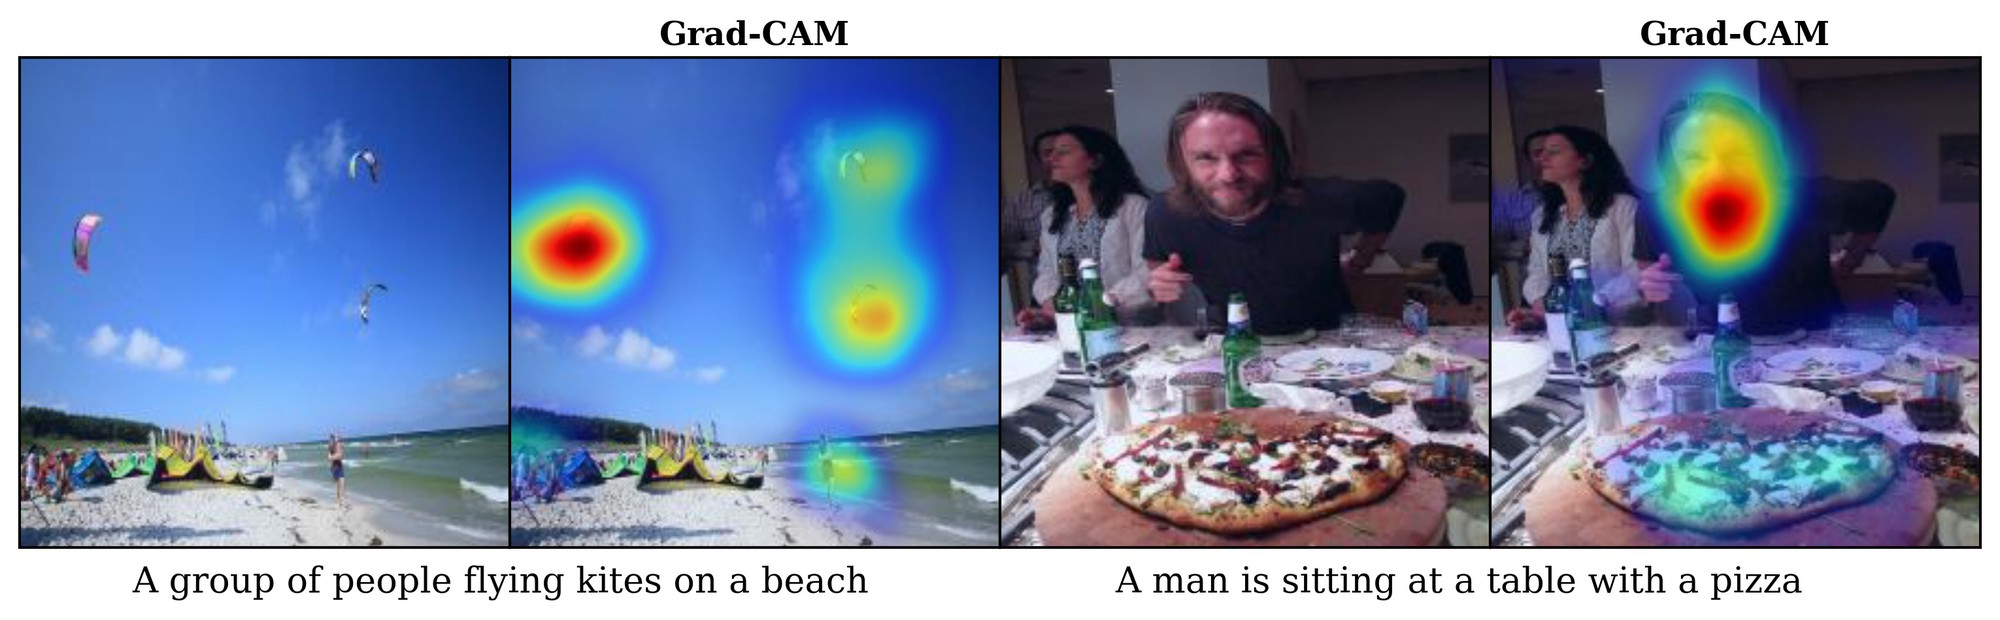
\includegraphics[width=\textwidth]{figures/captioning_main.jpg}
    \caption{\scriptsize{Image captioning explanations}}
  \label{fig:captioning}
  \end{subfigure}
  ~
    \begin{subfigure}[t]{0.49\textwidth}
    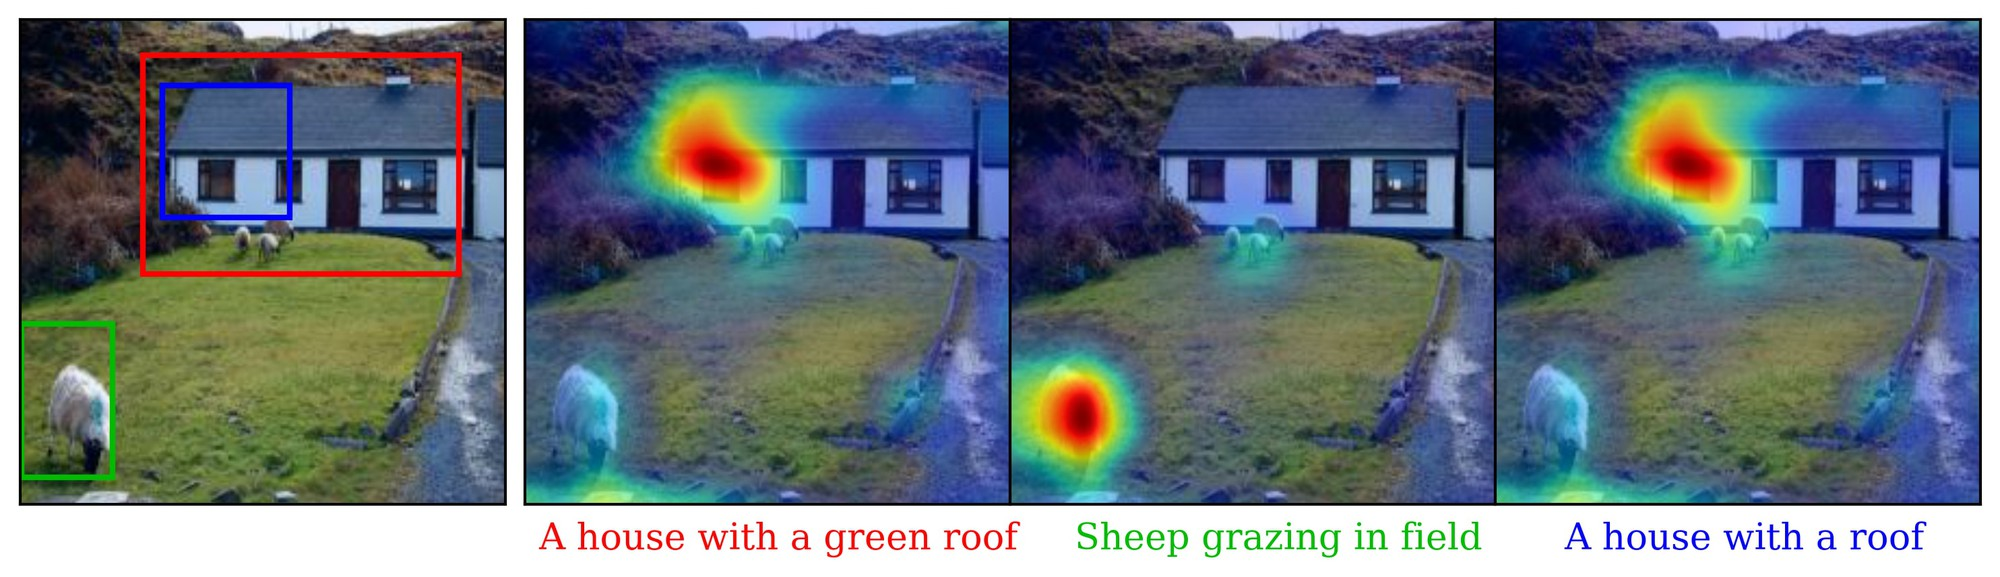
\includegraphics[width=\textwidth]{figures/densecap_main.jpg}
    \caption{\scriptsize{Comparison to DenseCap}}
   \label{fig:densecap}
   \end{subfigure}
   \vspace{14pt}
    \caption{Interpreting image captioning models: We use our class-discriminative localization technique, \gcam{} to find spatial support regions for captions in images. \reffig{fig:captioning} Visual explanations from image captioning model~\cite{karpathy2015deep} highlighting image regions considered to be important for producing the captions. \reffig{fig:densecap} \gcam{} localizations of a \emph{global} or \emph{holistic} captioning model for captions generated by a dense
    captioning model~\cite{johnson_cvpr16} for the three bounding box proposals marked on the left. We can see that we get back \gcam{} localizations (right) that agree with those bounding boxes -- even though the captioning model and Grad-CAM techniques do not use any bounding box annotations.}
\end{figure*}

\begin{figure*}[h]
\begin{center}
\begin{subfigure}[t]{\columnwidth}
\hspace{-20pt}
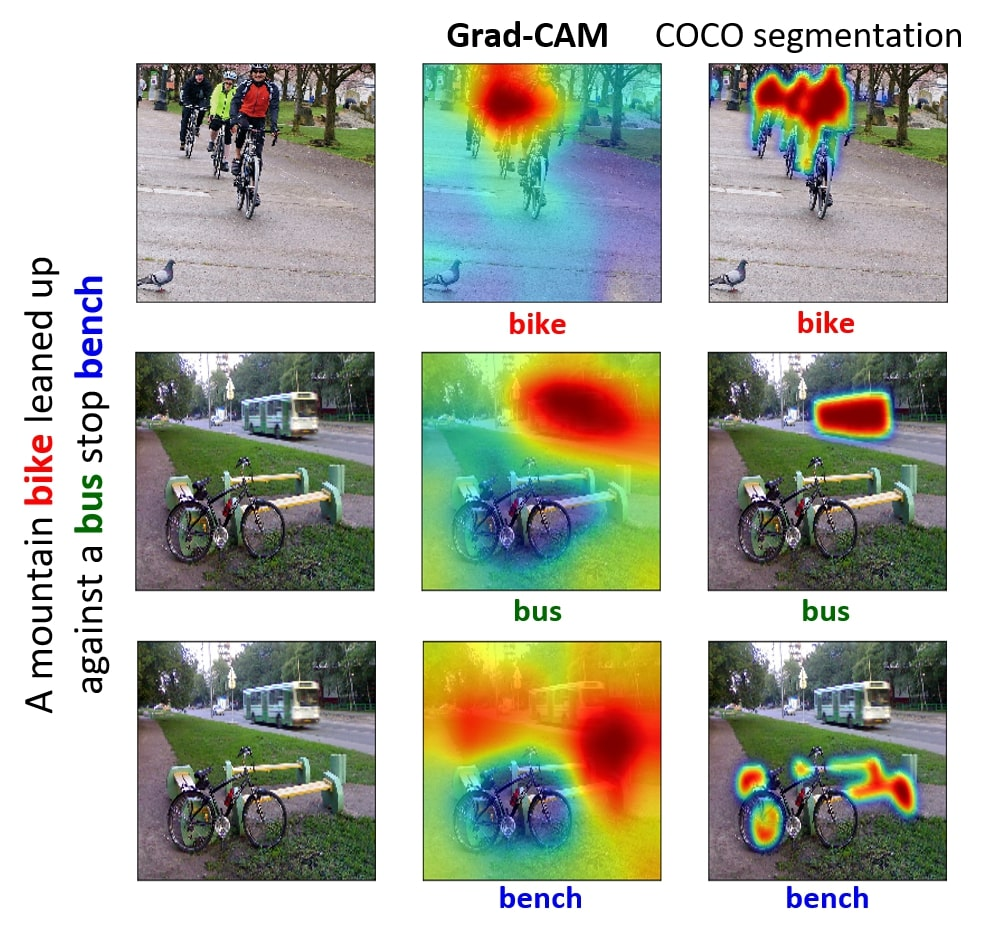
\includegraphics[scale=0.25]{figures/bike_bus_bench_show_tell.jpg}\caption{}
\vspace{10pt}
\end{subfigure}
\begin{subfigure}[t]{\columnwidth}
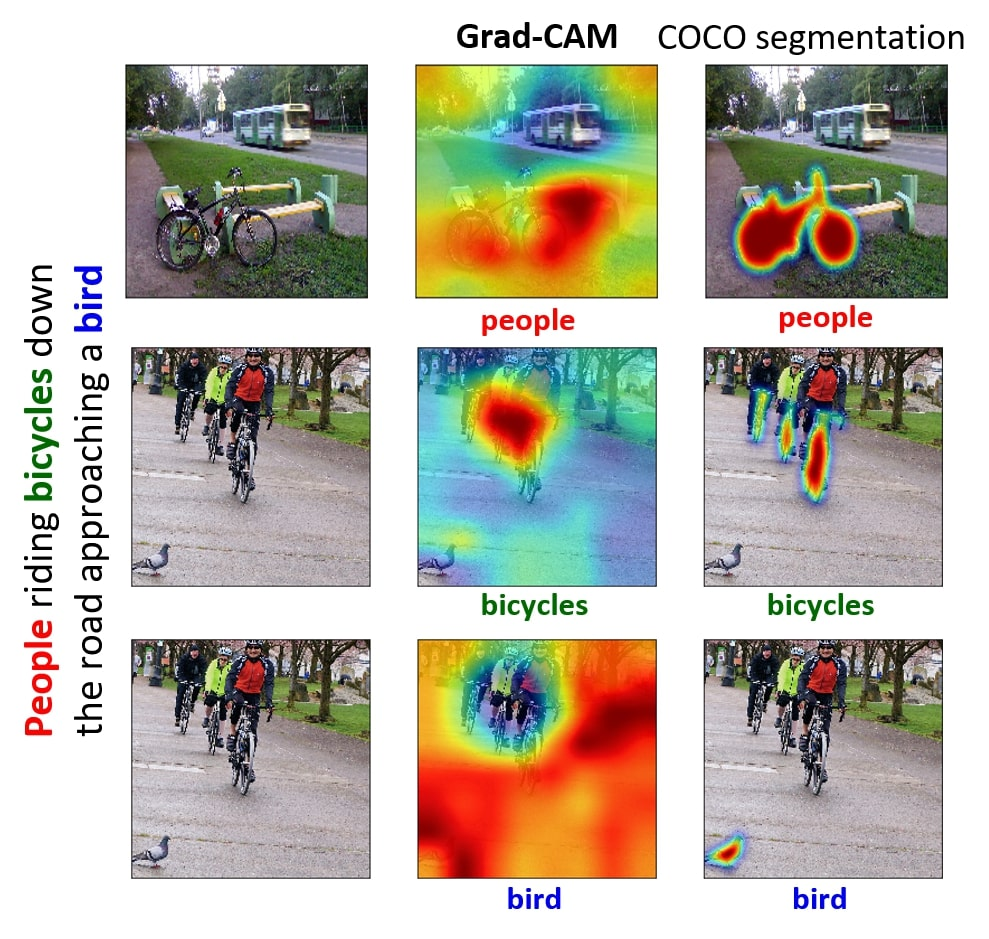
\includegraphics[scale=0.25]{figures/people_bicycles_bird_show_tell.jpg}\caption{}
\vspace{10pt}

\end{subfigure}
\caption{\rpi{Qualitative Results for our word-level captioning experiments: (a) Given the image on the left and the caption, we visualize \gcam{} maps for the visual words ``bike", ``bench" and ``bus". Note how well the \gcam{} maps correlate with the COCO segmentation maps on the right column. (b) shows a similar example where we visualize \gcam{} maps for the visual words ``people", ``bicycle" and ``bird".}}
\label{fig:captioning_word}
\end{center}
\end{figure*}

\vspace{-10pt}
\section{\gcam{} for Image Captioning and VQA}
Finally, we apply \gcam{} to vision \& language tasks such as image captioning~\cite{chen2015microsoft,johnson_cvpr16,vinyals_cvpr15}
and Visual Question Answering (VQA)~\cite{antol2015vqa,gao2015you,malinowski_iccv15,ren_nips15}.
We find that \gcam{} leads to interpretable visual explanations for these tasks
as compared to baseline visualizations which do not change noticeably across changing predictions.
Note that existing visualization techniques either are not class-discriminative
(\gb{}, \dec{}), or simply cannot be used for these tasks/architectures,
or both (CAM, c-MWP).

\vspace{-10pt}
\subsection{Image Captioning}\label{sec:nic}

  In this section, we visualize spatial support for an image captioning model using \gcam{}.
  We build \gcam{} on top of the publicly available neuraltalk2\footnote{\url{https://github.com/karpathy/neuraltalk2}} implementation~\cite{karpathy2015deep} that uses a finetuned VGG-16 CNN for images and an LSTM-based language model. Note that this model does not have an explicit attention mechanism.
  Given a caption, we compute the gradient of its log probability~\wrt units in the last convolutional layer of the CNN ($conv5\_3$ for VGG-16) and generate \gcam{} visualizations as described in \secref{sec:approach}.
See \reffig{fig:captioning}.
In the first example, \gcam{} maps for the generated caption localize
every occurrence of both the kites and people despite their relatively small size.
In the next example, \gcam{} correctly highlights the pizza and the man, but ignores the woman nearby, since `woman' is not mentioned in the caption. More examples are in \refsec{sec:sup_experiments}.%

\noindent \para{Comparison to dense captioning}
Johnson~\etal~\cite{johnson_cvpr16} recently introduced the Dense Captioning (DenseCap) task that requires a system to jointly localize and caption salient regions in a given image.
Their model consists of a Fully Convolutional Localization Network (FCLN)
that produces bounding boxes for regions of interest
and an LSTM-based language model that generates associated captions, all in a
single forward pass.
Using DenseCap, we generate \iccv{5 region-specific captions per image with associated ground truth bounding boxes.
\gcam{} for a whole-image captioning model (neuraltalk2) should localize the bounding box
the region-caption was generated for, which is shown in \reffig{fig:densecap}.
We quantify this by computing the ratio of mean activation inside \vs
outside the box. Higher ratios are better because they indicate stronger
attention to the region the caption was generated for.
Uniformly highlighting the whole image results in a baseline ratio of $1.0$ whereas
\gcam{} achieves $3.27$ $\pm$ $0.18$. Adding high-resolution detail gives an improved
baseline of $2.32$ $\pm$ 0.08 (\gb{}) and the best localization at $6.38$ $\pm$ 0.99 (\cgb{}).
Thus, \gcam{} is able to localize regions in the image that the
DenseCap model describes, even though the holistic captioning model was never
trained with bounding-box annotations.}

\vspace{-30pt}
\rpi{\subsubsection{Grad-CAM for individual words of caption}}

\rpi{In our experiment we use the Show and Tell model \cite{vinyals_cvpr15} pre-trained on MSCOCO without fine-tuning through the visual representation obtained from Inception \cite{szegedy2016rethinking} architecture. 
In order to obtain \gcam{} map for individual words in the ground-truth caption we one-hot encode each of the visual words at the corresponding time-steps and compute the neuron importance score using Eq. \eqref{eq:alpha1} and combine with the convolution feature maps using Eq. \eqref{eq:gcam}. 
}

\vspace{5pt}
\noindent
\rpi{\textbf{Comparison to Human Attention}~
We manually created an object category to word mapping that maps object categories
like $<$person$>$ to a list of potential fine-grained labels like
[“child”, “man”, "woman", ...]. 
We map a total of 830 visual words existing in COCO captions to 80 COCO categories.
We then use the segmentation annotations for the 80 categories as human attention for this subset of matching words.
}

\rpi{We then use the pointing evaluation from \cite{zhang2016top}. 
For each visual word from the caption, we generate the \gcam{} map and then extract the maximally activated point. 
We then evaluate if the point lies within the human attention mapsegmentation for the corresponding COCO category, thereby counting it as a hit or a miss. 
The pointing accuracy is then calculated as \\$Acc = \frac{\#Hits}{\#Hits+\#Misses}$. 
We perform this experiment on 1000 randomly sampled images from COCO dataset and obtain an accuracy of 30.0\%. 
Some qualitative examples can be found in \reffig{fig:captioning_word}. 
}










\vspace{10pt}
\subsection{Visual Question Answering}\label{sec:vqa}

Typical VQA pipelines ~\cite{antol2015vqa,gao2015you,malinowski_iccv15,ren_nips15}
consist of a CNN to process images and an RNN language model for questions.
The image and the question representations are fused to predict the answer,
typically with a $1000$-way classification ($1000$ being the size of the answer space).
Since this is a classification problem, we pick an answer (the score $y^c$ in \eqref{eq:scores})
and use its score to compute \gcam{} visualizations over the image to explain the answer.
Despite the complexity of the task, involving both visual and textual components,
the explanations (of the VQA model from Lu~\etal~\cite{Lu2015}) described in \reffig{fig:vqa} are surprisingly intuitive and informative.
\iccv{We quantify the performance of \gcam{} via correlation with occlusion maps,
as in \secref{sec:occ}. \gcam{} achieves a rank correlation (with occlusion maps)
of 0.60 $\pm$ 0.038 whereas \gb{} achieves 0.42 $\pm$ 0.038, indicating higher
faithfulness of our \gcam{} visualization.}




\begin{figure}[t]
    \begin{subfigure}[t]{\columnwidth}
    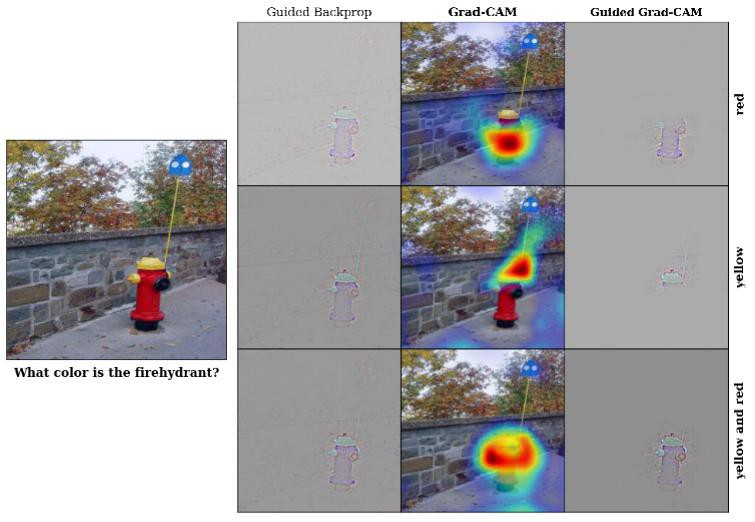
\includegraphics[scale=0.315]{figures/vqa_main_fig.jpg}
    \vspace{5pt}
    \caption{\scriptsize{Visualizing VQA model from \cite{Lu2015}}}
    \vspace{35pt}
    \label{fig:vqa_main_fig}
    \end{subfigure}
    \begin{subfigure}[t]{\columnwidth}
    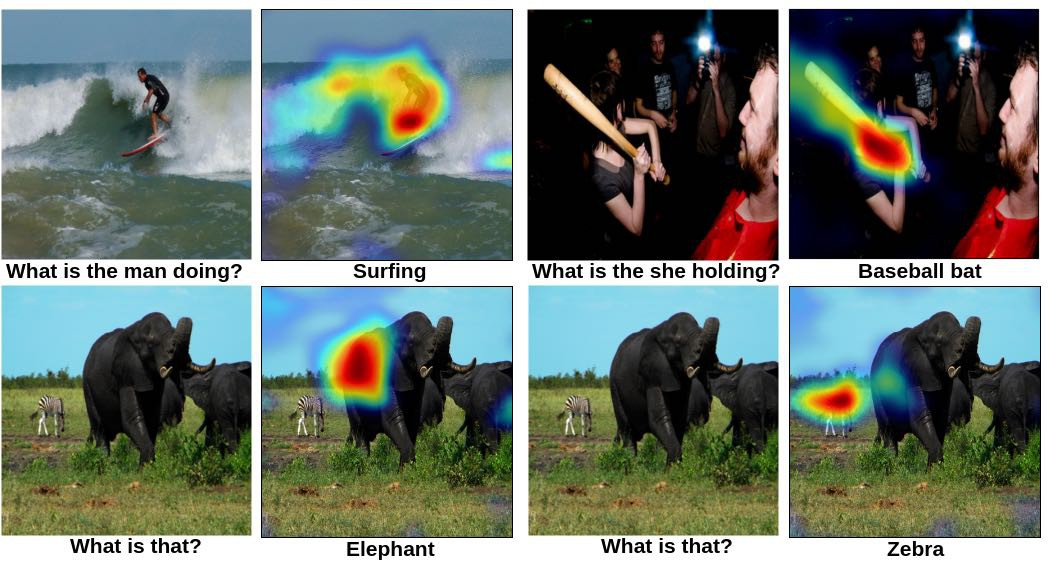
\includegraphics[scale=0.225]{figures/vqa_residual_main.jpg}
    \vspace{10pt}
    \caption{\scriptsize{Visualizing ResNet based Hierarchical co-attention VQA model from \cite{Lu2016}}}
    
        \label{fig:vqa_residual_main}
    \end{subfigure}
	\vspace{14pt}
    \caption{Qualitative Results for our VQA experiments: (a) Given the image on the left and the question ``What color is the firehydrant?'', we visualize \gcam{}s and \cgb{}s for the answers ``red", ``yellow" and ``yellow and red".
        \gcam{} visualizations are highly interpretable and help explain any target prediction -- for ``red'', the model focuses on the bottom red part of the firehydrant; when forced to answer ``yellow'', the model concentrates on it`s top yellow cap, and when forced to answer ``yellow and red", it looks at the whole firehydrant! \rp{ (b) Our approach is capable of providing interpretable explanations even for complex models.}
    }
	\label{fig:vqa}
\end{figure}
\noindent \para{Comparison to Human Attention}
Das~\etal~\cite{vqahat} collected human attention maps for a subset of the VQA dataset~\cite{antol2015vqa}.
These maps have high intensity where humans looked in the image in order to answer a visual question.
Human attention maps are compared to \gcam{} visualizations for the VQA model from~\cite{Lu2015}
on 1374 val question-image (QI) pairs from ~\cite{antol2015vqa} using the rank correlation evaluation protocol as in ~\cite{vqahat}.
\gcam{} and human attention maps have a correlation of 0.136, which is higher than chance or random attention maps (zero correlation).
This shows that despite not being trained on grounded image-text pairs, even non-attention based
CNN + LSTM based VQA models are surprisingly good at localizing regions for predicting a particular answer.

\noindent \para{Visualizing ResNet-based VQA model with co-attention}
    Lu~\etal~\cite{Lu2016} use a 200 layer ResNet~\cite{he_cvpr15} to encode the image, and jointly learn a hierarchical attention mechanism on the question and image. \reffig{fig:vqa_residual_main} shows \gcam{} visualizations for this network.
    \mac{As we visualize deeper layers of the ResNet, we see small changes in \gcam{}
    for most adjacent layers and larger changes between layers that involve dimensionality reduction.}
    \rpi{More visualizations for ResNets can be found in \refsec{sec:sup_resnet_analysis}}.
    To the best of our knowledge, we are the first to visualize decisions from ResNet-based models.





    
